\chapter{Validación de la Implementación y Experimentos}\label{chapter:implementation}

En este capítulo se detalla la implementación de la solución analizando un caso de prueba paso a paso, describiendo en cada uno de estos el proceso seguido al detalle. Para este caso de prueba estaremos usando el modelo Llama3.3-70b debido a que la experiencia en pruebas previas ha mostrado que este modelo es el que mejor tiempo de respuesta tiene.

Para este caso estaremos utilizando un dataset llamado \href{https://huggingface.co/datasets/sayanroy058/Business-Sales/viewer}{\textbf{Business-Sales}}, el cual representa datos de transacciones de ventas de automóviles. Este dataset resulta ideal para evaluar la capacidad del modelo Llama3.3-70b, tanto en la generación de informes automáticos como en la resolución de consultas en lenguaje natural.

\subsubsection{Consideraciones Iniciales sobre el Dataset}
Antes de describir las características principales del dataset, es fundamental destacar algunos aspectos críticos que afectan su procesamiento y análisis:
\begin{itemize}
	\item{Datos Faltantes:}
	Existen valores faltantes en algunas columnas, lo que requiere que el LLM analice e implemente alguna tecnica de imputacion para completar los valores faltantes.
	
	\item{Columnas Irrelevantes:}
	Algunas columnas, como VIN, contienen información única para cada vehículo y no aportan valor para los análisis o reportes generales. Por lo tanto, el modelo deberia darse cuenta de esto y ya sea desecharla en el preprocesamiento o por lo menos no utilizarla a la hora de recibir informacion.
	
	\item{Columnas con Abreviaturas:}
	Existen columnas como MMR (Manheim Market Report) cuyo significado no es explícito. El modelo deberá razonar en contexto para comprender su relevancia y cómo utilizarla en el análisis.
	
	\item{Interpretación de Rangos:}
	Algunas columnas, como condition, presentan valores numéricos cuya interpretación no es inmediata, ell modelo debera inferir sobre el rango y significado de estos valores para obtener resultados adecuados.
	
	\item{Razonamiento sobre Datos Heterogéneos:}
	Las columnas combinan datos categóricos, numéricos y textuales, lo que pone a prueba la capacidad del modelo para generalizar y extraer patrones útiles.
	
	\item{Gran cantidad de datos:}
	El dataset cuenta con cerca de 600 mil entradas lo cual hace que rea imposible pasarse completamente como contexto de niguno de los modelos de lenguajes en la actualidad.
\end{itemize}

\section{Interfaz}
Cuando accedemos al sitio web que nos proporciona streamlit cuando ejecutamos el programa nos encontramos con Nos encontramos con una pagina web que consta de dos columnas principales, una columna central mas espaciosa que seria el contenido principal de lapagina y una columna lateral a la izquierda que seria la columna de configuracion.

\subsection{Columna de configuracion}
La columna de configuracion es una pequeña columna lateral que nos permite cofugurar que modelo de los que nos provee la API de Groq vamos a estar utilizando ademas de un slider que nos permite seleccionar la cantidad de tokens maximos a generar por el model. Esto nos permite un mayor control sobre los llamados de la API y poder mantenernos dentro de los limites que nos impone el sitio web.

Esta columna ademas cuenta con un checkbox que por defecto se encuentra desabilitado llamado Debug, el cual si lo activamos nos abre una nueva columna a la derecha de la collumna principal con el contenido paso a paso de todo lo que se va realizando. En esta columna se muestran las llamadas y las respuestas del LLM, los resultado de las ejecuciones de los codigos generados, el proceso de preprocesado detallando cada una de las tareas que se identificaron y practicamente todo lo que va ocurriendo mientras se va generando el reporte.

\subsection{Culumna Principal}
La culumna principan cuenta con un encabezado con el nombre \textbf{Generador de Reportes Automatizados con LLM} y bajo este un componente de carga de archivo, que permite tanto la carga mediante la interfaz de carga de archivo propia de cada sistema operativo como la facilidad de simplementa arrastrar y soltar un archivo para su carga. Una vez que se carga el archivo comienza el proceso de extraer los datos relevantes del mismo.

A partir de los datos de informacion obtenidos anteriormente se le pide al LLM que cree una lista de tareas de preprocesado, dichas tareas pueden ir desde tareas predefinidas como marcar una columna como categorica o convertir una columna con fechas a objetos de fecha de python, a tareas mas complejas para las cuales se le pide que proporcione el codigo pandas correspondiente. En el caso que estamos analizando la lista de tareas que el modelo ejecuto fueron las siguientes:


\definecolor{jsoncolor}{rgb}{0.12,0.55,0.82}

\begin{lstlisting}
		{"tarea": "convertir_fecha", "columna": "saledate"}, 
		{"tarea": "identificar_categorica", "columna": "make"}, 
		{"tarea": "identificar_categorica", "columna": "model"}, 
		{"tarea": "identificar_categorica", "columna": "trim"}, 
		{"tarea": "identificar_categorica", "columna": "body"}, 
		{"tarea": "identificar_categorica", "columna": "transmission"}, 
		{"tarea": "identificar_categorica", "columna": "state"}, 
		{"tarea": "identificar_categorica", "columna": "condition"}, 
		{"tarea": "identificar_categorica", "columna": "color"}, 
		{"tarea": "identificar_categorica", "columna": "interior"}, 
		{"tarea": "identificar_categorica", "columna": "seller"}, 
		{"tarea": "filtrar", "columna": "vin", "sugerencia": "Eliminar columna, no se utiliza para el analisis"}, 
		{"tarea": "filtrar", "columna": "odometer", "sugerencia": "Filtrar valores outliers"}, 
		{"tarea": "filtrar", "columna": "condition", "sugerencia": "Filtrar valores outliers"}, 
		{"tarea": "filtrar", "columna": "mmr", "sugerencia": "Eliminar filas con datos faltantes"}, 
		{"tarea": "filtrar", "columna": "sellingprice", "sugerencia": "Eliminar filas con datos faltantes"}, 
		{"tarea": "pandas", "codigo": "df = df[df.condition < 50] # Filtrar condicion extrema"}, 
		{"tarea": "pandas", "codigo": "df = df[df.odometer < 50000] # Filtrar kilometraje extremo"}, 
		{"tarea": "pandas", "codigo": "df = df[df.mmr > 0] # Filtrar valores negativos de MMR"}, 
		{"tarea": "pandas", "codigo": "df = df[df.sellingprice > 0] # Filtrar valores negativos de precio de venta"} ]
\end{lstlisting}

Como podemos ver el modelo genero un json con un arreglo de tareas de preprocesado a realizar, destacando entre estas eliminar la columna vin, valores de precion de venta negaticvos y valores de condicion extrema. Esto nos permite ver que el proceso de extraccion de informacion que realizamos anteriormente dio buenos resultados ya que el modelo ha podido inferir las columnas relevantes, el rango en que estas se comportan y que valores pudieran ser 'ruido' en el dataset.

Una vez que se realize el preprocesamiento se le notificara al usuario el resultado del mismo si fue satisfactori o ocurrio algun error, en cualquier caso aparecera bajo estas notificaciones un cuadro de texto donde se le pide que inserte una consulta. La consulta debe ser en lenguaje natural y relacionada con el documento que se acaba de subir. Ademas se le sugiere al usuario 3 posibles consultas a realizar teniendo en cuenta el documento subido.

Para probar las capacidades del LLM le pediremos que haga un reporte de ventas de la marca Kia en el 2014. Esta consulta nos permitira ver si el modelo es capza de filtrar los datos que necesita para elaborar la respuesta, asi como si puede generar graficos relevantes que acompañen la informacion antes recibida.

\section{Generando el reporte}
Cuando cargamos el documento y este termina de ser preprocesado le hacemos la siguiente consulta:

\textit{Como se comportaron las ventas de kia en 2014 en relacion a las del año anterior}

A lo cual el primer paso que da el modelo es generar el \textbf{esqueleto del reporte}, donde para cada sección debe ademas del nombre de la sección proporcionar una descripción y alguna información de la como estructurar los gráficos o alguna sugerencia de como deberían ser o que datos debe mostrar.

En este caso el modelo nos proporcionó el siguiente esqueleto:

\noindent\colorbox{gray!5}{ % Fondo gris muy claro
	\noindent\fbox{ % Cuadro
		\begin{minipage}{\dimexpr\linewidth-2\fboxsep-2\fboxrule\relax}
			\begin{description}
				\item[\textbf{Sección Introducción}]
				\begin{itemize}
					\item \textbf{Descripción:} Breve contexto del análisis de las ventas de Kia en 2014 y comparación con 2013
					\item \textbf{Información:} Contexto general del análisis de ventas
				\end{itemize}
				\item[\textbf{Sección Ventas de Kia en 2014}]
				\begin{itemize}
					\item \textbf{Descripción:} Presentación detallada de las ventas de Kia en 2014
					\item \textbf{Información:} Datos numéricos de ventas en 2014. Sugerencia: Tabla detallada
				\end{itemize}
				\item[\textbf{Sección Ventas de Kia en 2013}]
				\begin{itemize}
					\item \textbf{Descripción:} Presentación detallada de las ventas de Kia en 2013
					\item \textbf{Información:} Datos numéricos de ventas en 2013. Sugerencia: Tabla detallada
				\end{itemize}
				\item[\textbf{Sección Comparación de Ventas entre 2013 y 2014}]
				\begin{itemize}
					\item \textbf{Descripción:} Comparación de las ventas de Kia en 2013 y 2014
					\item \textbf{Información:} Gráfico de barras para comparar las ventas en 2013 y 2014. Sugerencia: Gráfico de barras
				\end{itemize}
				\item[\textbf{Sección Análisis de la Tendencia de las Ventas}]
				\begin{itemize}
					\item \textbf{Descripción:} Análisis de la tendencia de las ventas de Kia en 2014 en comparación con 2013
					\item \textbf{Información:} Análisis de la tendencia de las ventas (aumento, disminución o estabilidad)
				\end{itemize}
				\item[\textbf{Sección Conclusiones y Recomendaciones}]
				\begin{itemize}
					\item \textbf{Descripción:} Resumen de los hallazgos y conclusiones del análisis de las ventas de Kia en 2014
					\item \textbf{Información:} Resumen de los hallazgos y conclusiones
				\end{itemize}
			\end{description}
		\end{minipage}
}}

A partir de este esqueleto, se empiezan a generar el reporte seccion por seccion. El primer paso para crear la seccion como habiamos planteado en el capitulo anterior es obtener datos del dataframe mediante un codigo python generado por el LLM. En esta ocasion el modelo genero el siguiente codigo.


\begin{lstlisting}
	import pandas as pd
	
	# Suponemos que el dataframe 'df' ya esta cargado
	
	# Calculamos el numero de ventas de Kia en 2014 y 2013
	ventas_2014 = len(df[(df['year'] == 2014) & (df['make'] == 'Kia')])
	ventas_2013 = len(df[(df['year'] == 2013) & (df['make'] == 'Kia')])
	
	# Calculamos el porcentaje de aumento o disminucion de ventas
	if ventas_2013 != 0:
	porcentaje_cambio = ((ventas_2014 - ventas_2013) / ventas_2013) * 100
	else:
	porcentaje_cambio = 0
	
	# Creamos un diccionario con la informacion necesaria para la seccion de introduccion
	response = {
		'ventas_2014': ventas_2014,
		'ventas_2013': ventas_2013,
		'porcentaje_cambio': porcentaje_cambio,
		'relevancia': 'El analisis de las ventas de Kia en 2014 y 2013 es relevante para entender el comportamiento del mercado y la estrategia de la empresa en ese periodo.'
	}
	
	print(response)
\end{lstlisting}

Notese que el modelo esta identificando correctamente que es lo que queremos y que datos necesitamos para esta introduccion, en este caso decidio obtener el numero total de ventas de ambos años y el porcentaje de cambio de un año al otro. El modelo ademas tuvo una ligera impresicion en este codigo ya que returna tambien un string de relevancia, el  cual parece ser una anotacion para generar el reporte donde destaca que el analisis de venta de estos anos es relevante para obtener el comportamiento del mercado.

El segundo paso para la generacion de una seccion era identificar y generar graficos que pudieran servir para un mejor anlisis por parte del usuario para los datos antes recogido. En esta ocasion el modelo luego de generar un codigo erroneo en primera instancia, fue capaz de generar los siguientes graficos.

\begin{figure}[H] % Usamos h! para forzar la posición aquí si es necesario, pero considera htbp para más flexibilidad
	\centering % Centrar todo el conjunto de figuras horizontalmente
	\begin{minipage}{0.48\textwidth} % Ajusta el ancho según necesites (ej. 0.48 para dejar espacio entre figuras)
		\centering
		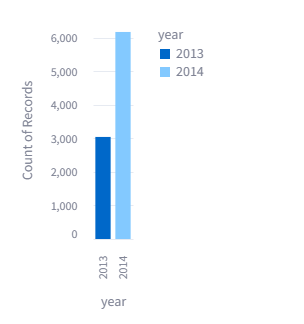
\includegraphics[height=150px]{grafica_anual.png} % Reemplaza con tu archivo real
		\caption{Número total de ventas de Kia por año}
		\label{fig:ejemplo_introduccion_grafico_anual}
	\end{minipage}
	\begin{minipage}{0.48\textwidth} % Ajusta el ancho según necesites
		\centering
		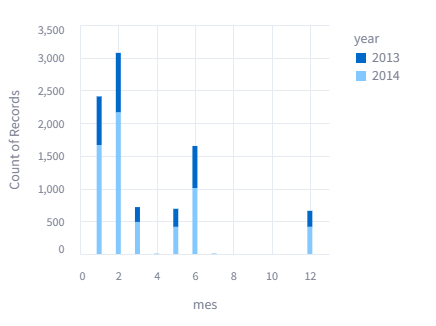
\includegraphics[height=150px]{grafica_mensual.png} % Reemplaza con tu archivo real
		\caption{Distribución de ventas de Kia por mes}
		\label{fig:ejemplo_introduccion_grafico_mensual}
	\end{minipage}
\end{figure}

Error detectado en la primera ejecucion del codigo generado
\textbf{\textit{Error message: Tz-aware datetime.datetime cannot be converted to datetime64 unless utc=True, at position 127}}

Luego cuando se le pide al modelo que utilizando los datos obtenidos y estos graficos genere la seccion del reporte, nos muestra ahora si en la columna principal la primera seccion del reporte.
//IMAGEN DE LA SECCION

A partir de aqui se generan el resto de secciones de la misma forma.